This section will first introduce the company Visual Solutions who provided the practical problem of integrating \gls{wrtc} with their own application for doing collaboration. Secondly I will give a quick overview of how the application Virtual Arena works by describing its underlying architecture, then I will look at some of the security concerns that occur when an enterprise collaboration system has to access the public internet.

\subsection{Visual Solutions}
Visual Solutions is a Norwegian company in the BB Visual Group\footnote{http://www.bbvisualgroup.com/}. Their primary business is within the integration of operations for the oil and gas industry. They create solutions enabling collaboration across organisation units and geographic locations. One of their applications Virtual Arena\cite{solutions_b2_virtual_2014}, which from now on will be referred to as VA, is a powerful and interactive tool that allows for high-performance application sharing, with audio and video communication from a 3D shared scene as seen in Figure \ref{fig:vsva-3d-scene}. VA supports many-to-many collaborative scenarios by utilizing a media server which will be described in the next section.
\\
\begin{figure}[here]
\centerline{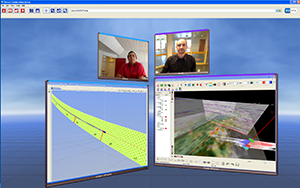
\includegraphics[scale=0.6]{virtualarena.png}}
\caption{Virtual Arena 3D shared scene}
\label{fig:vsva-3d-scene}
\end{figure}

\subsection{Virtual Arena}
VA is the application that Visual Solutions has created for doing visual collaboration over IP. The architecture of VA is visualized in Figure \ref{fig:vsva-architecture}. The application uses a media server that serves multiple purposes. It acts as a \gls{mcu}, applies mitigation strategies for scenarios with limited bandwidth, and also sharing of applicaton data. Mitigation strategies can f.ex be reducing the video bitrate to adjust and adapt for poor connections. The media server works together with a router for distributing the streams. By utilizing a media server VA can support a lot of incoming and outgoing streams. A client can subscribe to multiple streams of audio/video and applications. It manages these connections using a tree structure, but this is an advanced topic that I won't go into detail about. In the next subsections the different parts of the architecture in Figure \ref{fig:vsva-architecture} will be described with the necessary information required to understand the practical problem this thesis will try to solve.

\begin{figure}[here]
\centerline{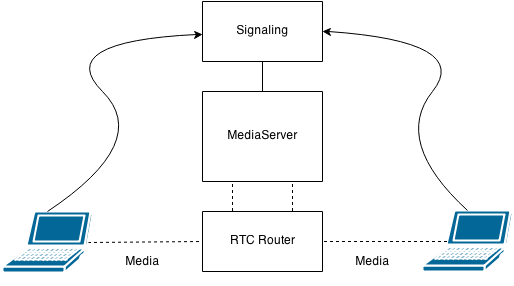
\includegraphics[scale=0.6]{enterprise-mcu-architecture.png}}
\caption{Virtual Arena systems architecture}
\label{fig:vsva-architecture}
\end{figure}

\subsubsection{Signaling}
VA has a proprietary way of doing signaling over \gls{rtcp}. RTCP is a control protocol for \gls{rtp}. This is where the clients send messages to the media server describing which streams they want to subscribe to. Communication between peers and the media server is done by opening up ports in the firewall to listen for incoming TCP and UDP connections. These ports are preconfigured for this application. The media server can receive incoming streams and route it to all peers connected. The streams are identified using a \gls{ssrc}, which is defined in the header packets of the RTP streams.

\subsubsection{Transport}
VA uses raw RTP streams over UDP. This is basically the standard protocol used for transmitting real-time media in any communication system. There will be more details about this protocol in the upcoming sections.

\subsubsection{Media}
VA uses patent-free codecs for audio and video. It uses Speex for audio, and Theora for video. The Speex codec is designed for high quality speech and low bitrate, which is perfect for audio communications. It supports both narrowband and wideband sampling rates in the same bit-stream\cite{speex}, which allows for minimizing bandwidth and an adaptable sound quality. The Theora codec is a common choice in enterprise systems, it is less CPU-intensive than the popular H.264 codec\cite{theora}, which is licensed by Cisco. Theora is also license free, however H.264 offers the added benefits of hardware acceleration in a lot of graphic cards, and Cisco has recently announced that they will make H.264 open-source\cite{h264-free}, which will effectively make the codec free to use in technologies like \gls{wrtc}.

\subsection{Security}
VA only uses raw RTP streams, because no security is needed. It operates in a closed business environement, so transport level encryption is not necessary, because unidentified peers are not allowed inside the network anyways. The enterprise firewall has very strict polices, only allowing certain kinds of traffic on specific ports. VA enforce this by using a DMZ??? It works like this....

\subsection*{Summary}
VA operates very much like a typical enterprise comunication system. It uses common transport protocols and codecs, however it's architecture is still very different from the protocols and codecs defined in \gls{rtcweb}, which we will see in the next section.